\chapter{Equilibrio de mercado y sistemas de ecuaciones}
\label{cap:equilibrio}

\section{El mercado como encuentro de dos fuerzas}

Un mercado pone en contacto a quienes quieren comprar (demanda) con quienes quieren vender (oferta). Cada lado reacciona al precio en sentido contrario: los compradores quieren precios bajos, los vendedores precios altos. La pregunta económica clásica es: \emph{¿existe un precio que concilie ambos deseos?} La respuesta es el \textbf{equilibrio de mercado}, una de las ideas más potentes de toda la economía y, según \cite{mankiw}, el verdadero «caballo de batalla» del análisis.

\begin{definicion}[Equilibrio de mercado]
El mercado está en \emph{equilibrio} en el par $(p^{*},q^{*})$ donde la cantidad demandada iguala a la ofrecida:
\[
Q_d(p^{*}) = Q_s(p^{*}) = q^{*}.
\]
A $p^{*}$ se lo llama \emph{precio de equilibrio} y a $q^{*}$ \emph{cantidad de equilibrio}.
\end{definicion}

La intuición del ajuste es la siguiente. Si el precio estuviera por encima de $p^{*}$, habría \emph{exceso de oferta} (sobra mercadería) y los vendedores bajarían precios. Si estuviera por debajo, habría \emph{exceso de demanda} (faltan productos, hay cola) y el precio subiría. Solo en $p^{*}$ no hay presión a moverse: por eso es un equilibrio.

\section{Resolver el equilibrio: un sistema de dos ecuaciones}

Encontrar el equilibrio es \textbf{resolver un sistema de ecuaciones}. Con la demanda \eqref{eq:demanda} y la oferta \eqref{eq:oferta}:
\begin{equation}
\begin{cases}
Q_d = a - b\,p \\[2pt]
Q_s = c + d\,p
\end{cases}
\qquad\Longrightarrow\qquad a - b\,p = c + d\,p .
\end{equation}
Igualando demanda y oferta y despejando, el precio de equilibrio es
\begin{equation}
p^{*} = \frac{a-c}{b+d}, \qquad\text{y luego}\qquad q^{*} = a - b\,p^{*}.
\label{eq:p_equilibrio}
\end{equation}

Esta es la versión más simple de un \textbf{sistema lineal}. Cuando los modelos crecen —varios mercados interconectados, varios bienes, restricciones— el sistema tiene más ecuaciones y más incógnitas, y conviene escribirlo en forma \emph{matricial} $A\mathbf{x}=\mathbf{b}$ y resolverlo con álgebra lineal, como veremos con Leontief en el Capítulo~\ref{cap:leontief}. La lógica, sin embargo, es siempre la misma: tantas ecuaciones independientes como incógnitas.

\begin{ejemplo}[Equilibrio en el mercado de un bien]
Sea $Q_d = 120 - 2p$ y $Q_s = -30 + 3p$. Igualando:
\[
120 - 2p = -30 + 3p \;\Longrightarrow\; 150 = 5p \;\Longrightarrow\; p^{*} = 30.
\]
La cantidad de equilibrio es $q^{*} = 120 - 2(30) = 60$. A un precio de \$30 se compran y venden exactamente 60 unidades, y el mercado se «vacía» sin sobrantes ni faltantes.
\end{ejemplo}

\begin{figure}[htbp]
\centering
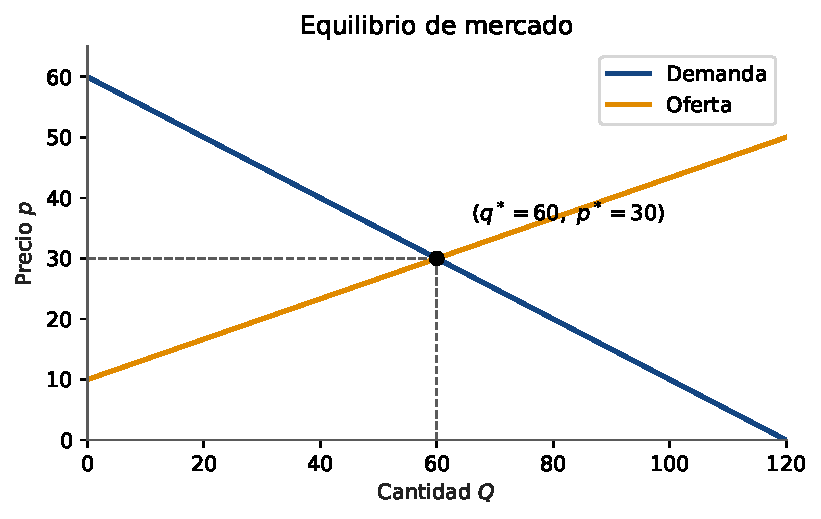
\includegraphics[width=0.72\linewidth]{figuras/equilibrio}
\caption{El equilibrio es la intersección de oferta y demanda. Por encima de $p^{*}$ sobra producto y el precio baja; por debajo, falta y el precio sube.}
\label{fig:equilibrio}
\end{figure}

\section{Estática comparativa: ¿qué pasa si algo cambia?}

El verdadero valor del equilibrio para la gestión no es el número en sí, sino poder responder \textbf{«¿qué pasaría si\ldots?»}. A este ejercicio se lo llama \emph{estática comparativa}: comparamos el equilibrio antes y después de un cambio en algún parámetro \cite{chiang}.

Por ejemplo, un impuesto específico de $t$ pesos por unidad cobrado al productor desplaza la oferta: ahora los vendedores necesitan $t$ pesos más por cada unidad, de modo que la oferta pasa a $Q_s = c + d(p - t)$. Recalculando \eqref{eq:p_equilibrio} se obtiene cómo cambian $p^{*}$ y $q^{*}$, y por lo tanto quién «paga» realmente el impuesto (la \emph{incidencia}). Este tipo de análisis —cambiar un parámetro y recomputar el equilibrio— es exactamente lo que las herramientas computacionales hacen sin esfuerzo, permitiendo explorar decenas de escenarios en segundos.

\begin{ideabox}
\textbf{Por qué importa.} El equilibrio convierte una pregunta de gestión vaga («¿conviene este precio?») en un cálculo reproducible. Y la estática comparativa convierte el modelo en una \emph{herramienta de simulación}: cambio un supuesto y veo el efecto. Esa es, en una frase, la promesa de los métodos cuantitativos aplicados.
\end{ideabox}

\begin{labbox}
En la notebook, resolver $Q_d = Q_s$ es una línea: \texttt{sympy.solve(Qd - Qs, p)}. La computadora despeja $p^{*}$ simbólicamente —sin que tengamos que hacer el álgebra a mano— y luego evalúa $q^{*}$. Para la estática comparativa basta cambiar un parámetro y volver a llamar a \texttt{solve}: el sistema de ecuaciones de \eqref{eq:p_equilibrio} se vuelve un experimento interactivo.
\end{labbox}

\section{Síntesis del capítulo}

El equilibrio de mercado surge de igualar oferta y demanda, lo que en términos matemáticos es resolver un sistema de ecuaciones. La estática comparativa nos permite estudiar el efecto de impuestos, subsidios o cambios de costos. En el próximo capítulo generalizamos la idea de «resolver sistemas» al caso de una economía con muchos sectores interdependientes: el modelo de Leontief.
